\chapter{Experiments on Synthetic Graphs}

The methodology described is applied to two classes of synthetic networks. These generated benchmarks allow for the comparison to the ground truth communities, and also test how well each algorithm can extract community structures as the ratio of inter and intra edges increases, obfuscating the embedded classes. A test is also performed on networks of fixed inter/intra connection ratio, but with increasing size, to test the ability to extract communities effectively as the size of the network increases.

\section{Girvan-Newmann Experiments}
Here we present the results of each algorithm for a range of parameter sets on the Girvan-Newmann benchmark for a number of parameter sets for each of the selected algorithms. Graphs were constructed with the average external degree $k_{out}$  of each node between 1 and 8. As the average total degree of a node in the Girvan-Newmann benchmark is 16, a value of $k_{out}\geq8$ means that there is no strong community structure present.


%%table            parameter set 1 | parameter set 2 | parameter set 3 | parameter set 4 | parameter set  5
% mixing parameter


%% convergence curves


\begin{figure}
	\begin{tabular}{cc}
		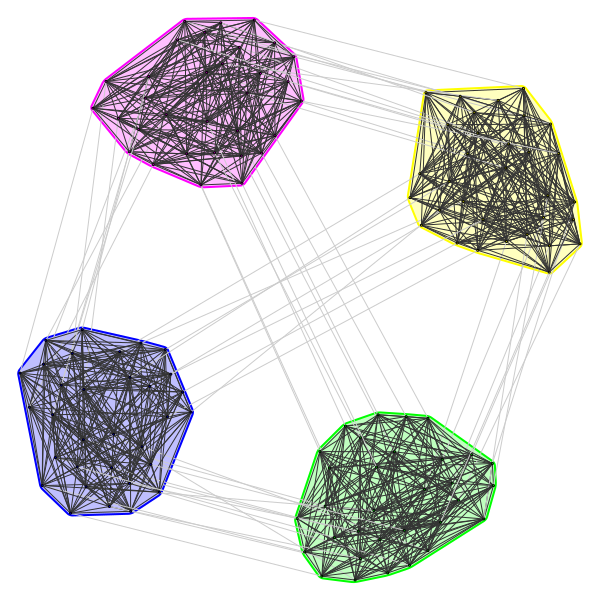
\includegraphics[width=65mm]{images/girvan_kout_1_0.png} &   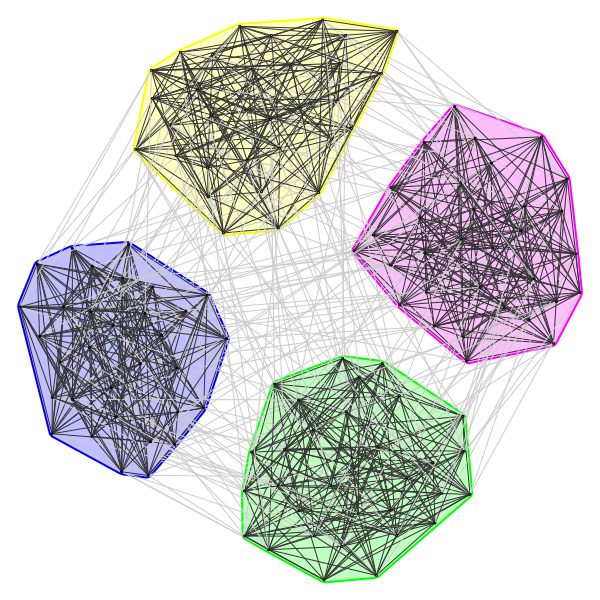
\includegraphics[width=65mm]{images/girvan_kout_3_0.png} \\
		(a) $k_{out}=1$ & (b) $k_{out}=3$ \\[6pt]
		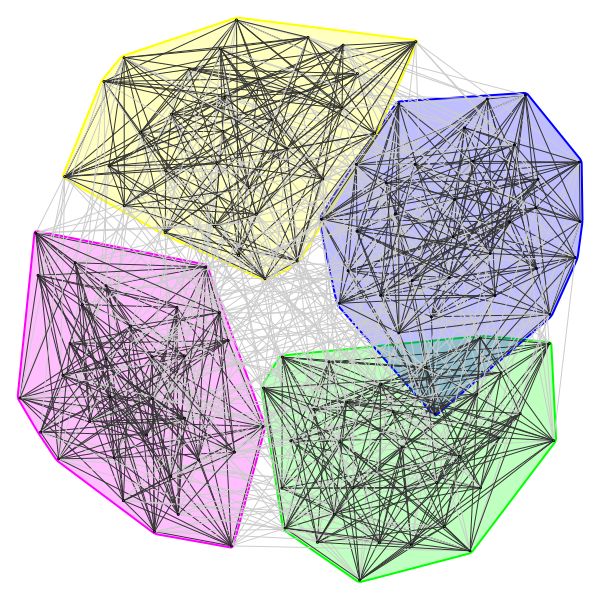
\includegraphics[width=65mm]{images/girvan_kout_5_0.png} &   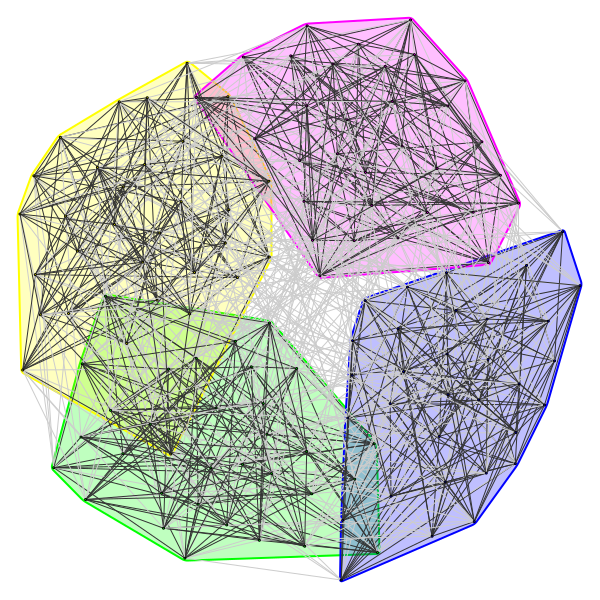
\includegraphics[width=65mm]{images/girvan_kout_6_0.png} \\
		(c) $k_{out}=5$ & (d) $k_{out}=6$ \\[6pt]
		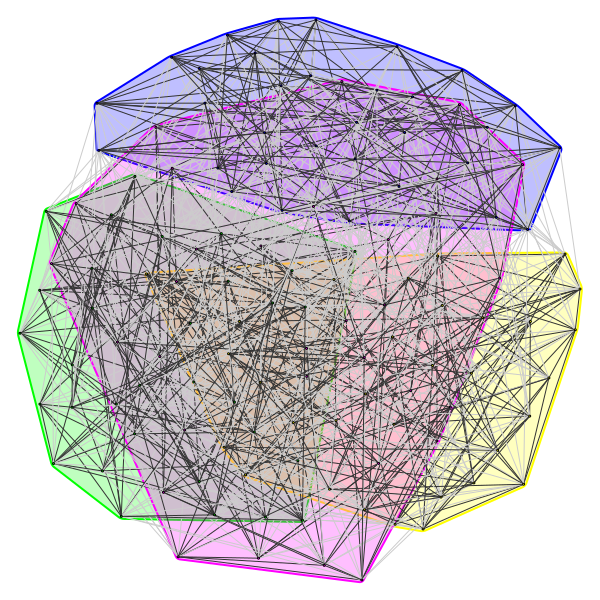
\includegraphics[width=65mm]{images/girvan_kout_8_0.png} &   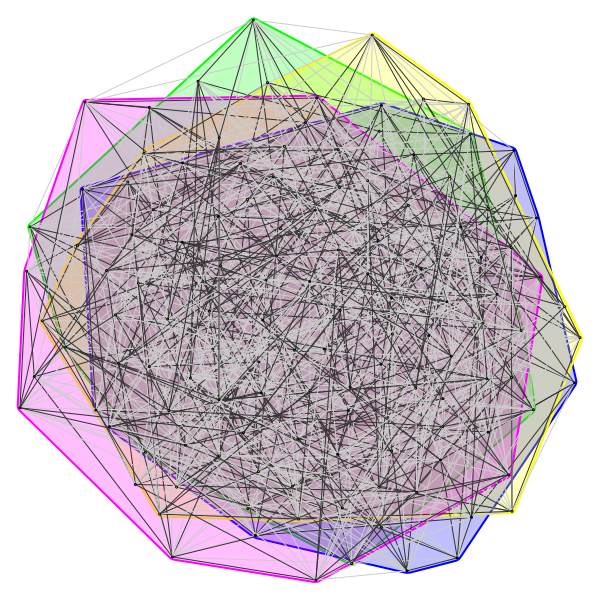
\includegraphics[width=65mm]{images/girvan_kout_10_0.png} \\
		(c) $k_{out}=8$ & (d) $k_{out}=10$ \\[6pt]
		
	\end{tabular}
	\caption{Visualizations of the GN benchmark with increasing $k_{out}$ parameters.}
\end{figure}


%% non-parametric tests

\section{LFR Benchmarks With Increasing Mixing \\ Parameter}
While the Girvan-Newmann benchmark allows for creating networks with increasingly difficult to identify communities, it is limited by its limits in terms of a fixed degree distribution, and no variance in community size. The LFR benchmark extends the planted $\ell$-partition model to allow a degree distribution following the power law and a variety of community sizes. 

Four sets of graphs were generated, with mixing parameters ranging from 0.1 to 0.6. The parameters used are summarized in table \ref{lfrparam}.

%%table            parameter set 1 | parameter set 2 | parameter set 3 | parameter set 4 | parameter set  5
% mixing parameter
\begin{table}[h!]
	\centering
	\begin{tabular}{|l | l| l | l | l | l |} 
		\hline
		\multicolumn{1}{|c|}{\textbf{Group}} & 
		\multicolumn{1}{|c|}{\textbf{$N$}}  &  
		\multicolumn{1}{|c|}{\textbf{$k$}}  &  
		\multicolumn{1}{|c|}{\textbf{$max_k$}} &
		\multicolumn{1}{|c|}{\textbf{$min_c$}} & 
		\multicolumn{1}{|c|}{\textbf{$max_c$}}\\
		\hline
		\hline
		1000\_s & 1000 & 20 & 50 & 10 & 50\\ 
		\hline
		1000\_b & 1000 & 20 & 50 & 10 & 100\\ 
		\hline
		5000\_s & 5000 & 20 & 50 &10 & 50\\ 
		\hline
		5000\_b & 5000& 20 & 50 & 10 & 100\\
		\hline
	\end{tabular}
	\caption{Parameters used to generate the LFR benchmarks. Each group was generated with the mixing parameter $\mu$ ranging from 0.1 to 0.6}
	\label{lfrparam}
\end{table}

%% lfr graph images


%% convergence curves

%% Extracted communities

%% non-parametric tests



\section{LFR Benchmarks With Increasing Size}
While an effective algorithm should detect communities even as the definition becomes more and more unclear from inter-community links, it should also be able to detect communities as the network scales in size. For this experiment, we use the parameter sets selected for each algorithm for the experiments on increasing mixing parameter for consistency.
%% convergence curves

%% Extracted communities

%% non-parametric tests
